\documentclass[10pt,journal,cspaper,compsoc]{IEEEtran}

\usepackage{graphicx}
\usepackage{amsmath}
\usepackage{url}
\usepackage{mathabx}
% \usepackage{amssymb}
% \usepackage{afterpage}
\title{Simulation and Modeling Experiments}
\author{\IEEEauthorblockN{
  Aayush Lamichhane\IEEEauthorrefmark{1},
  Bishal Katuwal\IEEEauthorrefmark{2},
  Bishant Baniya\IEEEauthorrefmark{3}, and
  Gobind Prasad Sah\IEEEauthorrefmark{4}}\\
\IEEEauthorblockA{Department of Electronics and Computer Engineering, IOE Pulchowk Campus\\
Patan, Lalitpur\\
Email: \IEEEauthorrefmark{1}075bct005.aayush@pcampus.edu.np,
\IEEEauthorrefmark{2}075bct028.bishal@pcampus.edu.np,
\IEEEauthorrefmark{3}075bct030.bishant@pcampus.edu.np,
\IEEEauthorrefmark{4}075bct038.gobind@pcampus.edu.np,
}}
\date{\today}

\begin{document}
\maketitle

\begin{abstract}
  This report presents the results of five simulation and modeling experiments conducted in both MATLAB and Python. The experiments cover a broad range of topics, including the simulation of a chemical reaction system, an R-C amplifier circuit, the generation of random numbers, the modeling of a mass spring damper system and a national econometric system. The simulations were conducted using mathematical models and software tools, and the results were analyzed and compared with theoritical data, whenever possible. These experiments demonstrate the importance and applications of simulation and modeling in engineering and science, and provide valuable insights into the behavior and performance of complex systems under different scenarios.
\end{abstract}

\section{Introduction}
Simulation and modeling are powerful tools for analyzing and predicting the behavior of complex systems in engineering and science under various scenarios. By creating mathematical models of real-world phenomena, the behaviour of complex systems under different conditions can be simulated. The results provided by simulation can be used to gain insights into the underlying mechanisms of the system. This helps to make predictions about future behavior of the system under consideration.

The remainder of this report is organized as follows. Sections 2 to 6 present the codes, results and discussion regarding the experiments. Section 7 provides a summary of the experiments and their results, and discusses the implications of the findings.

\section{Experiment 1 : Simulation of the chemical reaction}
\subsection{Objectives}
  \begin{itemize}
    \item To develop the mathematical modeling of the continuous system.
    \item To determine the state of the system i.e. the value of reactants and product at different point of
    time.
  \end{itemize}
  \subsection{Methodology}
  Chemical reactions exhibit dynamic equilibrium. At the steady state the rates of the forward and the backward reaction is same.
  in this study, we considered a reaction where two chemicals(C1 and C2) react together to form a third chemical(C3),
  \begin{equation}
    C1 + C2 = C3
  \end{equation} 
  The rate of reaction depends on a large number of factors such as 
  \begin{enumerate}
    \item Amount of C1 and C2 used.
    \item Temperature
    \item Pressure
    \item Humidity
    \item Catalyst
  \end{enumerate}
  For this study, we ignored all other parameters and assume the reaction to only depend on amount of chemicals.
  This allowed the simulation of chemical reaction using ordinary differential equations (ODEs) and/or partial differential equations (PDEs).
  The rate of increase of C1, C2 and C3 at any given instance is given by:
  \begin{equation}
    \frac{dC1}{dt} = K_{2} C3 - K_{1} C1 C2 
  \end{equation}
\begin{equation}
  \frac{dC2}{dt} = K_{2} C3 - K_{1} C1 C2
\end{equation}
\begin{equation}
  \frac{dC3}{dt} = 2 K_{1} C1 C2 - 2 K_{2} C3
\end{equation}

Considering C1(t), C2(t) and C3(t) as the concentration of C1, C2 and C3 at time t, the concentration at time 
\begin{math}
  t + \Delta t
\end{math}
is :
\begin{equation}
  C1(t+\Delta t) = C1(t) + \frac{dC1(t)}{dt} \Delta t
\end{equation} 
\begin{equation}
  C2(t+\Delta t) = C2(t) + \frac{dC2(t)}{dt} \Delta t
\end{equation}
\begin{equation}
  C3(t+\Delta t) = C3(t) + \frac{dC3(t)}{dt} \Delta t
\end{equation}
Using this methodology, the state of the system was simulated.
  \subsection{Results}
    Insert plot here

  \subsection{Discussion}
    The results of the first experiment showed that the state of the system is highly dependent on the initial concentration of the reactants. In the three cases we studied, forward reaction was preferred when the concentration of reactant was high and backward reaction was favoured when the concentration of product was high. Also comparatively, the reaction was faster when the concentration of the chemicals were higher.

\section{Experiment 2 : Simulation of the R-C amplifier circuit}
  \subsection{Objective}
  \begin{itemize}
    \item To develop the mathematical modeling of a continuous system.
  \end{itemize}
  \subsection{Methodology}
  In this study, a R-C amplifier circuit was modelled as a continuous system.
  Like with any continuous system, the circuit was modeled with the
  variables of the model representing the attributes controlled by continuous functions.
  The following circuit was represented mathematically by two differential equations.
  
  \begin{figure}[!h]
    \centering
    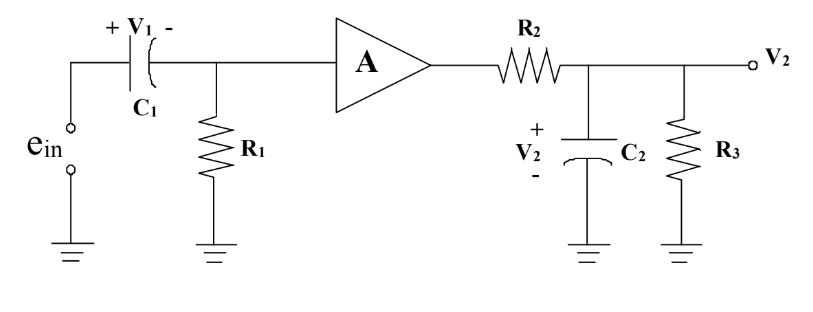
\includegraphics[scale = 0.5]{images/circuit.PNG}
    \caption{R-C Amplifier Circuit}
  \end{figure}

  Current entering through capacitor \begin{math}
    C_1
  \end{math} at the input side is:
  \begin{equation}
    C_1 \frac{dV_1}{dt} = (e_{in} - V)/R_1
  \end{equation}
  \begin{equation*}
    \frac{dV_1}{dt} = (e_{in}-V)/R_1C_1
  \end{equation*}
  Current entering through capacitor \begin{math}
    C_2
  \end{math} at the output side is:
  \begin{equation}
    C_2 \frac{dV_2}{dt} = \frac{A}{R_2(e_{in}-V1)} - \frac{V_2(R_2+R_3)}{R_2 R_3}
  \end{equation}
  Thus the equations for simulation was :
  \begin{equation}
    \frac{dV_1}{dt} = A_{11} * V_1 + B_1 * e_{in}
  \end{equation}
  \begin{equation}
    \frac{dV_2}{dt} = A_{21} * V_1 + A_{22} * V_2 + B_2 * e_{in}
  \end{equation}
  where,
  \begin{equation*}
    A_{11} = -1/(R_1C_1) = -B_1
  \end{equation*}
  \begin{equation*}
    A_{21} = -A/(R_2C_2) = -B_2
  \end{equation*}
  \begin{equation*}
    A_{22} = - (R_2 + R_3)/(R_2R_3C_2)
  \end{equation*}
  These values for \begin{math}
    V_1 and V_2
  \end{math}
  was solved by using Runge-Kutta-4 methods.
  \begin{equation*}
      m_1 = f(x_1,y_1)
  \end{equation*}
  \begin{equation*}
    m_2 = f(x_1 + h/2, y_1 + m_1 h/2)
  \end{equation*}
  \begin{equation*}
    m_3 = f(x_1 + h/2, y_1 + m_2 h/2)
  \end{equation*}
  \begin{equation*}
    m_4 = f(x_1 +h, y_1 + m_3 h)
  \end{equation*}
  \begin{equation*}
    y_{i+1} = y_i + ( (m_1 + 2m_2 + 2m_3 + m_4)/6)h
  \end{equation*}

\section{Experiment 3 : Generation of random number}
\subsection{Objective}
  \begin{itemize}
    \item To generate a Random number
  \end{itemize}
\subsection{Methodology}
  In this study, we generate a random number and use Chi-square test to veify the acceptance.
  The number is generated by Congruence method which is pseudorandom number generation. 
  In this method, we used a seed \begin{math}
    (r_o)
  \end{math} and two variables( a and b ) to generate the pseudorandom number.
  Considering P as the upper limit of random number, we got a random number in the closed interval.
  The mathematical model is given by :
  \begin{equation}
    r_{i+1} = (a * r_i + b) \%  P
  \end{equation}
  Here,
  \begin{itemize}
    \item a = 1, the method is additive.
    \item b = 0, the method is multiplicative.
    \item Else, the method is mixed. 
  \end{itemize}
  After generation of pseudorandom number, we used Chi-square test to verify the acceptance.
  Chi-square test is a frequency test given by,
  \begin{equation}
    \chi _o ^2 = \sum (O_i - E_i)^2 / E_i
  \end{equation}
  where 
  \begin{math}
    E_i = N/n
  \end{math}
  is the expected number.\\
  and \begin{math} O_i \end{math}  is the observed number.\\
  For given confidence level and degree of freedom, acceptance value is found out from table. If
the calculated value is grater than the table value, the numbers are accepted for their uniformity of distribution.
  
\section{Experiment 4 : Simulation of mass spring damper system}
\subsection{Objectives}
\begin{itemize}
  \item To develop the mathematical modeling of the (continuous system) mass spring damper system.
  \item To determine the state of the system i.e. x, distance moved at different point of time.
\end{itemize}  
\subsection{Methodology}
In this study, we make a mathematical model of a mass spring damper system. The physical system is as follows :
\begin{figure}[h!]
  \centering
  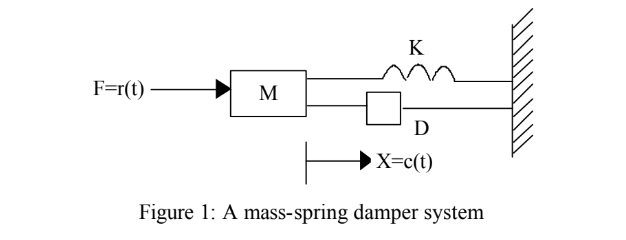
\includegraphics[scale= 0.7]{images/spring-mass.PNG}
  \caption{Mass-Spring damper system}
\end{figure}
The free body diagram of this system is :
\begin{figure}[h!]
  \centering
  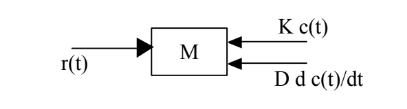
\includegraphics{images/sping_mass_freebody.PNG}
  \caption{Free-body diagram}
\end{figure}
 The mathematical model of this system can be derived from Newton's law of motion.
 \begin{equation*}
  M * \frac{d^2C(t)}{dt^2} = K r(t) - (D \frac{dC(t)}{dt} + K C(t))
 \end{equation*}
 or
 \begin{equation*}
  M * \frac{d^2C(t)}{dt^2} + D \frac{dC(t)}{dt} + K C(t) = Kr(t)
 \end{equation*}
 Thus, the mathematical model of a mass spring damper system with mass M, force r(t), damoer coefficient(D), spring coefficient(K) and displacement C(t) is given by: 
 \begin{equation}
  M * \frac{d^2C(t)}{dt^2} + D \frac{dC(t)}{dt} + K C(t) = Kr(t)
 \end{equation}
 which can be rewritten as :
 \begin{equation}
  \frac{d^2C(t)}{dt^2} + \frac{D}{M} \frac{dC(t)}{dt} + \frac{K}{M} C(t) = \frac{1}{M} Kr(t)
 \end{equation}
 This is the required mathematical model of the given mathematical system. Comparing equation 15 with general secibd order partial equation:
 \begin{equation}
  \frac{d^2x(t)}{dt^2} + 2 \xi W \frac{dx(t)}{dt} + W^2 x(t) = W^2 F
 \end{equation}
 where, Damping ratio  
 \begin{math}
  \xi = D/2 . M . W
 \end{math}
 \\Angular frequency of oscillation W = 
 \begin{math}
  \sqrt{K/M}
 \end{math} 
 \\We show how x varies in response to a steady force applied at time t = 0 for the various values of \begin{math}
  \xi .
 \end{math}
\section{Experiment 5 : Simulation of national econometric system}
\subsection{Objectives}
\begin{itemize}
  \item To develop the mathematical modeling of the national econometric system.
  \item To determine the state of the system at various fixed interval of time using distributed lag model
\end{itemize}
\subsection{Methodology}
  In this study, we model a national econometric system as a distributed lag model. Models that have the properties of changing only at fixed intervals of time, and of basing current values  of the variables on other current values and values that occurred in previous intervals, are called distributed lag models. Such type of models consists of linear algebra. They represent a continuous system, but one in which the data is only available at fixed
  points in time.

  For this study, following simple static mathematical model of nation econometric system is considered.
  \begin{equation}
    C = 20 + 0.7 (Y-T)
  \end{equation}
  \begin{equation}
    I = 2 + 0.1 Y
  \end{equation}
  \begin{equation}
    T = 0.2 Y
  \end{equation}
  \begin{equation}
    Y = C + I + G
  \end{equation} 
    where,\\
    C is Consumption\\
    I is Investment\\
    T is Taxes\\
    G is Government expenditure\\
    Y is national income\\

    This static model is made dynamic by picking a fixed time interval and expressing the
    current values of the variables in terms of values at previous interval. Any variables that appears in the form of its previous interval is said to be a lagged variable. Its values in a previous interval is denoted by attaching the suffix –1 to the variable. The static model can be made dynamic by lagging all the variables. To achieve this, we don't lag all the variables but rather we lag one variable(Y) and express all other in terms of that variable.
    Thus, above set of equations can be written as : 
    \begin{equation}
      Y = 45.45 + 2.27 (I + G)
    \end{equation}
    \begin{equation}
      I = 2 + 0.1 Y_(-1)
    \end{equation}
    \begin{equation}
      T = 0.2 Y
    \end{equation}
    \begin{equation}
      C = 20 + 0.7 ( Y - T )
    \end{equation}
    We have 5 variables (C,I,T,G,Y) and only 4 equations, thus we provide the value of G and solve the above equations. 
  \section{Conclusion}
  In conclusion, the five simulation experiments conducted in this study have demonstrated the potential of mathematical modeling and computer simulation in various fields of science and engineering. The simulation of chemical reaction has provided insights into reaction kinetics which can aid in the design of chemical reactors and optimization of chemical processes. The simulation of R-C amplifier circuit has shown the effectiveness of circuit analysis techniques and numerical methods in designing and analyzing electronic circuits. The generation of acceptable pseudo random numbers has importance in Monte Carlo simulations and stochastic modeling. The modeling of mass-spring-damper system has revealed the dynamic behavior of mechanical systems and the effects of damping and resonance on the system response. The simulation of national econometric system has demonstrated the usefulness of macroeconomic models in policy analysis and decision-making.  Overall, the study has provided valuable insights into the use of computational modeling and simulation in various applications and has highlighted the importance of numerical methods and simulation tools in modern science and engineering. 
\appendices
\section{MATLAB Code for Chemical Kinetics}

% \bibliographystyle{IEEEtran}
% \bibliography{references}

\end{document}